\documentclass{sig-alternate}
%%%%%%%%%%%%%%%%%%%%%%%%%%%%%%%%%%%%%%%%%%%%%%%%%%%%%%%%%%%%%%%%%%%%%%
% LATEX DEFINITIONS
%%%%%%%%%%%%%%%%%%%%%%%%%%%%%%%%%%%%%%%%%%%%%%%%%%%%%%%%%%%%%%%%%%%%%%

\usepackage{hyperref}
\usepackage{array}
\usepackage{graphicx}
\usepackage{booktabs}
\usepackage{pifont}
\usepackage{todonotes}
\usepackage{rotating}
\usepackage{color}

\newcommand*\rot{\rotatebox{90}}


%%%%%%%%%%%%%%%%%%%%%%%%%%%%%%%%%%%%%%%%%%%%%%%%%%%%%%%%%%%%%%%%%%%%%%
\begin{document}
%
% --- Author Metadata here ---
\conferenceinfo{WOODSTOCK}{'97 El Paso, Texas USA}
\CopyrightYear{2014} 
\crdata{X-XXXXX-XX-X/XX/XX}  % Allows default copyright data (0-89791-88-6/97/05) to be over-ridden - IF NEED BE.
% --- End of Author Metadata ---

\title{Sicientific Impact Metrics for XSEDE%
\titlenote{(Produces the permission block, and
copyright information). For use with
SIG-ALTERNATE.CLS. Supported by ACM.}}
\subtitle{[Extended Abstract]
\titlenote{A full version of this paper is available as
\texttt{www.acm.org/eaddress.htm}}}

\numberofauthors{4} 
\author{
\alignauthor
Gregor von Laszewski\titlenote{Corresponding Author.}\\
       \affaddr{Indiana University}\\
       \affaddr{2719 10th Street}\\
       \affaddr{Bloomington, Indiana, U.S.A.}\\
       \email{laszewski@gmail.com}
% 2nd. author
\alignauthor
Fugang Wang\\
       \affaddr{Indiana University}\\
       \affaddr{2719 10th Street}\\
       \affaddr{Bloomington, Indiana, U.S.A.}\\
% 3rd. author
\alignauthor
Geoffrey C. Fox\\
       \affaddr{Indiana University}\\
       \affaddr{2719 10th Street}\\
       \affaddr{Bloomington, Indiana, U.S.A.}\\
\and  % use '\and' if you need 'another row' of author names
% 4th. author
\alignauthor 
Tom Furlani\\
       \affaddr{CRC}\\
       \affaddr{Street}\\
       \affaddr{Buffalo NY, 47401}
}
\date{13 March 2014}


% A category with the (minimum) three required fields
%\category{H.4}{Information Systems Applications}{Miscellaneous}
%A category including the fourth, optional field follows...
%\category{D.2.8}{Software Engineering}{Metrics}[complexity measures, performance measures]

\terms{Theory}

\keywords{h-index, metric, FutureGrid, Technology audit, XSEDE}



%%%%%%%%%%%%%%%%%%%%%%%%%%%%%%%%%%%%%%%%%%%%%%%%%%%%%%%%%%%%%%%%%%%%%%
% TOC
%%%%%%%%%%%%%%%%%%%%%%%%%%%%%%%%%%%%%%%%%%%%%%%%%%%%%%%%%%%%%%%%%%%%%%

\tableofcontents

\newpage

%%%%%%%%%%%%%%%%%%%%%%%%%%%%%%%%%%%%%%%%%%%%%%%%%%%%%%%%%%%%%%%%%%%%%%
% LIST OF TODOS
%%%%%%%%%%%%%%%%%%%%%%%%%%%%%%%%%%%%%%%%%%%%%%%%%%%%%%%%%%%%%%%%%%%%%%

\listoftodos

\newpage

%%%%%%%%%%%%%%%%%%%%%%%%%%%%%%%%%%%%%%%%%%%%%%%%%%%%%%%%%%%%%%%%%%%%%%
% TITLE OF PAPER
%%%%%%%%%%%%%%%%%%%%%%%%%%%%%%%%%%%%%%%%%%%%%%%%%%%%%%%%%%%%%%%%%%%%%%

\pagenumbering{arabic}

\maketitle

%%%%%%%%%%%%%%%%%%%%%%%%%%%%%%%%%%%%%%%%%%%%%%%%%%%%%%%%%%%%%%%%%%%%%%
% ABSTRACT OF PAPER
%%%%%%%%%%%%%%%%%%%%%%%%%%%%%%%%%%%%%%%%%%%%%%%%%%%%%%%%%%%%%%%%%%%%%%


\begin{abstract}

TBD

\end{abstract}

%%%%%%%%%%%%%%%%%%%%%%%%%%%%%%%%%%%%%%%%%%%%%%%%%%%%%%%%%%%%%%%%%%%%%%
% SECTIONS
%%%%%%%%%%%%%%%%%%%%%%%%%%%%%%%%%%%%%%%%%%%%%%%%%%%%%%%%%%%%%%%%%%%%%%

\section{Introduction}

Science advancement and engineering discoveries have been requiring increasingly large amount of computing power, and many of them usually need very large-scale resources that cannot be efficiently managed by individual research groups. Dedicated big computing facilities play an important role here, in which resources are shared among various groups of researchers, while the facilities themselves are managed by dedicated staff. XSEDE, an evolution from the TeraGrid, for instance, provides large scale resources to researchers to advance science and expedite engineering discoveries \cite{www-xsede}. It is open to eligible researchers, while a research proposal submission is required. Upon approval of the proposal the researcher is granted a predefined amount of resources, e.g., computing core-hours, storage spaces, and support by staff. The resources represent a tremendous amount of investment, thus some natural questions try to figure out how such resources help: 

\begin{enumerate}
\item Is there a way to measure the impact of providing such facilities like XSEDE to scientist? 

\item How is the impact of scientific research of individual user, project, or field of study, with respect to the resources allocated? 

\item When evaluating a proposal request, what is the criteria to judge whether the proposal is potentially leading to good research and broader impact, and how to get metrics to back up this?
\end{enumerate}

To answer these questions, we need a process to quantify the scientific outcome for the individual research units, and then define metrics when correlating to the consumed resources to finally measure the impacts of the science activities conducted. In this paper, we present a framework that does this, while studying activities and their outcomes on XSEDE. For this paper we restrict our effort to those related to scientific publications as the base unit of the research output, and obtained data as well as derived various metrics on top of that to measure the impact of individual users, projects, Field of Science (FOS), and XSEDE itself in a whole.

In the following sections we will first briefly discuss the related works, and then present our designed framework and some implementation details. The results and discussions then follow. Finally, we outline our future plans and conclude the paper.



\section{requirements}

\section{system design}

\begin{figure}[htb]
  \centering
    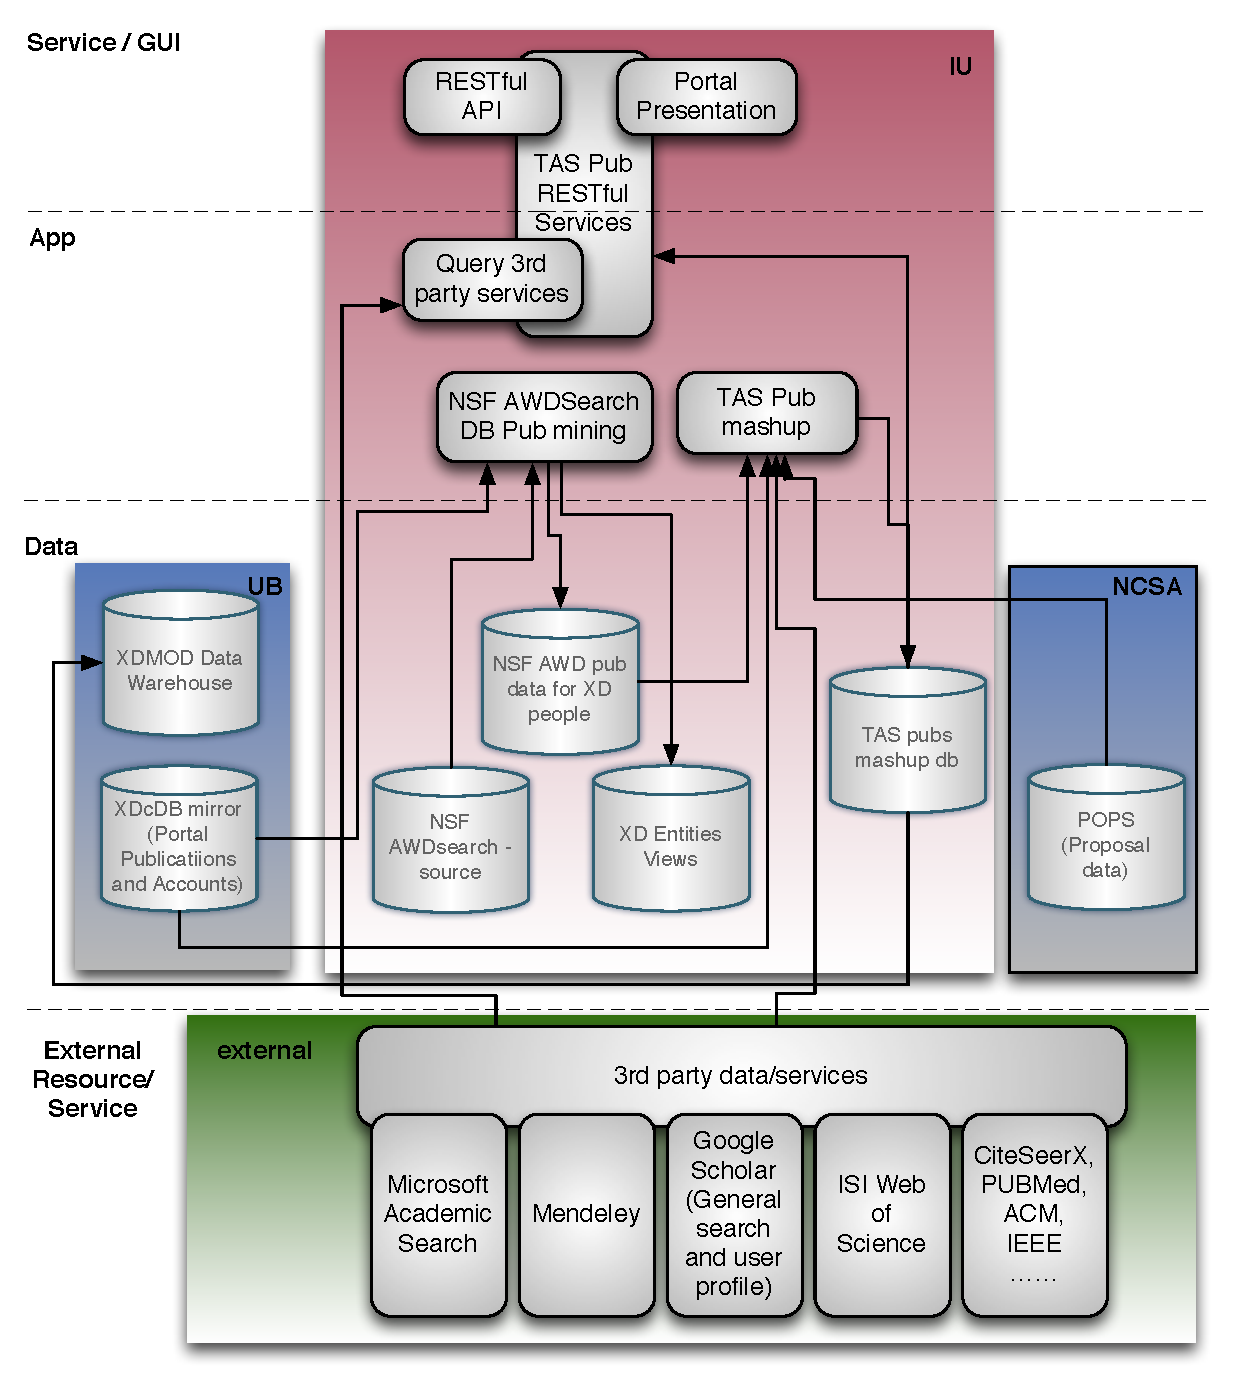
\includegraphics[width=1.0\columnwidth]{images/tas-arch.pdf}
  \caption{The Architecture of the Framework}\label{F:tas-arch}
\end{figure}
 
We have designed a software framework to support the impact measuring. It is a largely distributed (involves IU, UB, NCSA and other external resources e.g.) service-oriented system  that consists of publication and citation data retrieval (e.g., from Google Scholar and ISI Web of Science), parsing and processing while correlating data from various databases and services (e.g., XSEDE central database and POPS database); the metrics generation and analysis system for the different aggregated levels (users, projects, organization, Field of Science (FOS) ); as well as a presentation layer using a light weight portal in addition to exposing some data via RESTful API.

Fig \ref{F:tas-arch} shows the layered system architecture, with an emphasis on relationships between related components especially among the databases. In general we obtain the publication data for each XSEDE user, and then retrieve the citation data for each publication. The data are originally collected per user and per publication basis, but would be aggregated based on organization, XSEDE project/account, Field of Science (FOS), etc. for the metrics generation and analysis. When correlating the data to the input, in this context the Service Units (SUs) awarded by XSEDE, the analysis could reveal patterns and trends of how XSEDE can impact the sciences and potentially helps to achieve better return of investment.

While we are using the system to analyze the scientific impact of XSEDE, the framework itself is flexible enough that could be easily adapted to other similar systems for impact measure and analyses.


\section{Implementation}

We have implemented the system following best practices and leveraging popular tools and frameworks. The core system is in python. Python libraries MySQLdb, SQLAlchemy, psycopg2 are used to interact with the various data sources. Python library requests and BeautifulSoup are used in scraping citation data and properly parsing them. Flask framework is used for the service interface and Web GUI. Various JavaScript libraries such as highcharts are utilized in the web tier.

Publication and citation data retrieval is probably the foremost work so we detail the process in the following.

\subsection{Publication Data Acquisition}

\begin{figure}[htb]
  \centering
    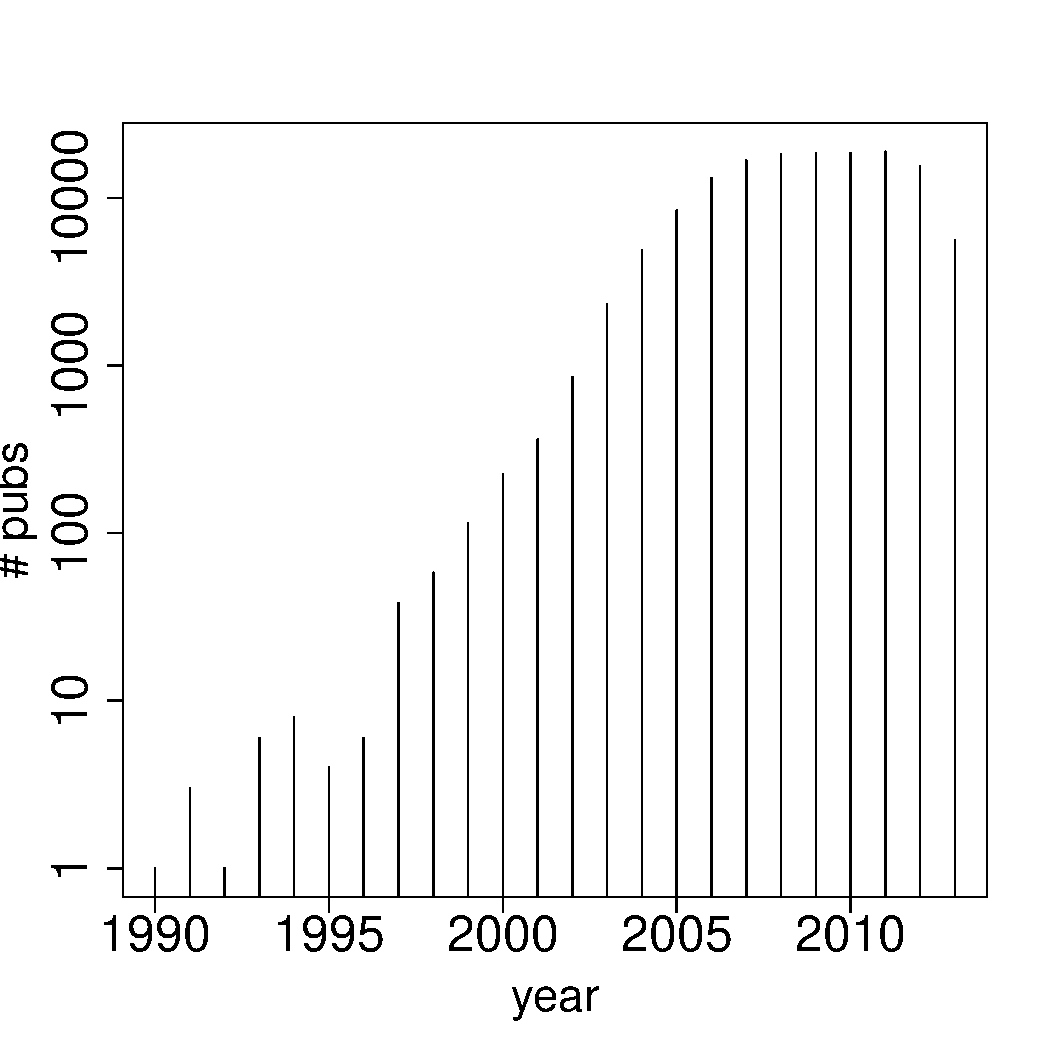
\includegraphics[width=1.0\columnwidth]{images/21_pubs_year_distribution.pdf}
  \caption{Publications by Year}\label{F:pubs-year-distribution}
\end{figure}

\begin{figure}[htb]
  \centering
    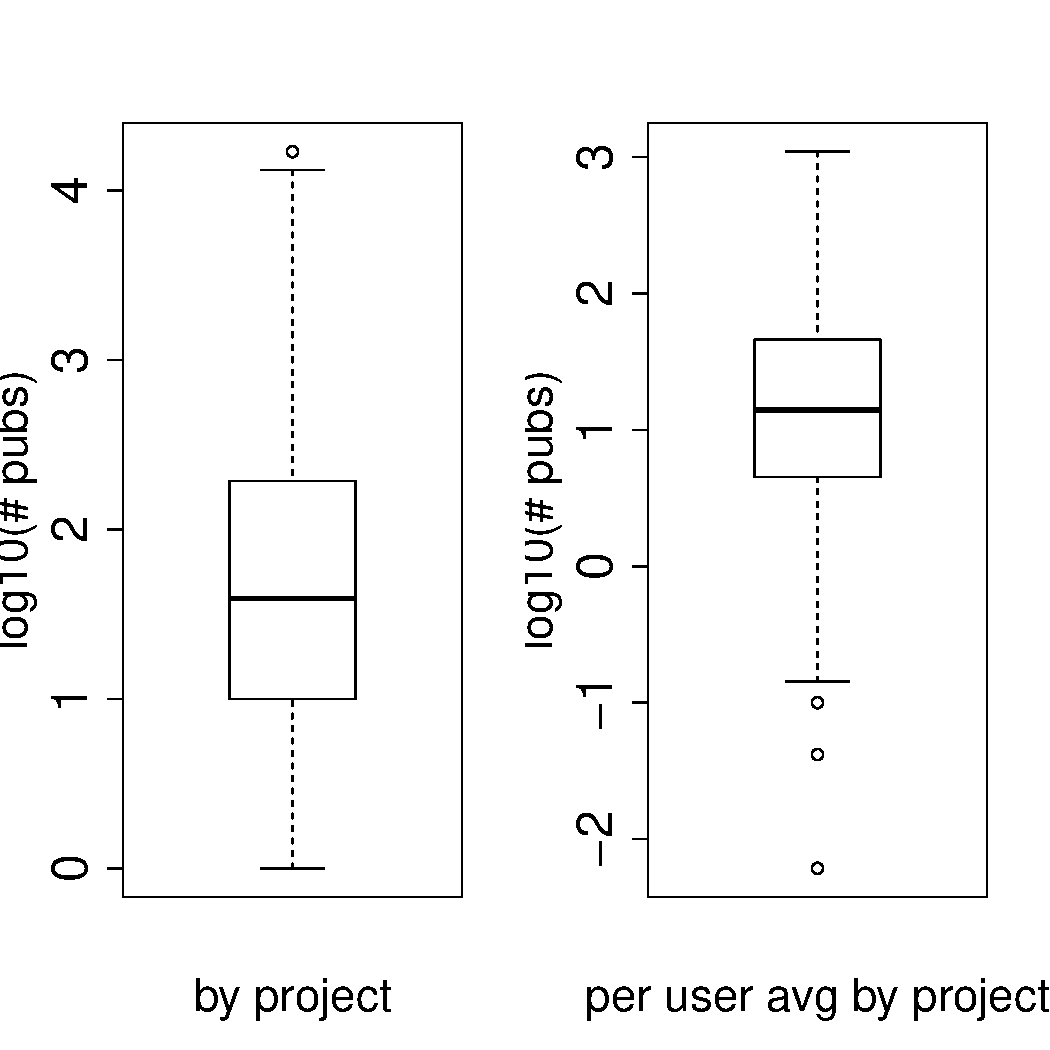
\includegraphics[width=1.0\columnwidth]{images/01_dist_npubs_proj.pdf}
  \caption{Distribution of number of publications}\label{F:dist-npubs-proj}
\end{figure}

We started the project by following the automated approach to obtain publication data. Publication citation data are available via subscribed resources such as ISI Web of Science \cite{www-isiwos} or open access such as Google Scholar \cite{www-googlescholar}, Microsoft Academic Search \cite{www-msas}, and Mendeley \cite{www-mendeley}, however they usually don't provide unlimited access.

Another approach which is probably more ideal is to get publication data from users. The user curated data tend to be more accurate comparing to automated mining, besides, there is another benefit that it gives extra information regarding a publication's association with the system, e.g., to which project it belongs. FutureGrid leveraged the drupal biblio module \cite{www-drupal-bib} with some customized design to support easy publication report and mass import via users or a staff member, and associated the publications with the related projects \cite{www-fgbiblio}. XSEDE now also provides a similar functionality via the portal \cite{www-xdportalpub}. nanoHUB citation analysis \cite{www-nanohubcite} as we have mentioned is also based on publication data submitted by users via a web form.

The framework itself supports pluggable data sources via mining databases and/or accessing 3rd party service APIs. We have experimented various data sources including Microsoft Academic Search, Google Scholar including user profile, and mining NSF award search data that are available upon request from NSF. The obtained data are then stored into the Mashup database which provides a common interface to other components in the system as well as collaborating systems like XDMOD.

In this study we focus only on two data sources - the user submitted data via XSEDE, and the NSF award search data for automated mining. The former source has user curated data with project affiliation information, thus it could give a measure on `direct' impact of XSEDE. However as it requires users' input, the former source currently has very limited data entries. The automated way obtains publication data for XSEDE users, which are not essentially direct output of using XSEDE resources, thus provides a measure on general or `indirect' impact of XSEDE. As a XSEDE user is affiliated with accounts/projects, and the projects are part of one or more FOS, we tag one publication as being related to the projects and FOSes based on these links. This is not most ideal but it provides a means to analyze the `indirect' impact on other levels in addition to users.

Based on the stated process, we were able to obtain over 142 thousand publication entries for over 20 thousand XSEDE users as of Jan 2014. Figure \ref{F:pubs-year-distribution} shows the yearly distribution of the publications. Figure \ref{F:dist-npubs-proj} shows distribution of number of publications by project (on the left) and by per user for each project.

\subsection{Citation Data Retrieval}

While for publication data user curated data might be more ideal, for citation data we have to go to the automated way for better accuracy and common grounds to compare. Google Scholar and ISI Web of Science provide such data, with some noticeable limitations. E.g., Google Scholar does not provide an API, nor it allows unlimited access within a bounded time period from one request source. ISI data does not impose a rate limiting while you have subscribed access, however it does not provide easy access API either. So one has to submit query via the web UI and then parse the data from the tabulated results list.

We have explored both approaches for a subset of the publication data, and did a comparison of the results. While similar comparison has been attempted \cite{yang2006citation} in a very small sample size - 2 people and about 100 publications, our study has included 33861 publications and 1462 users.

\begin{figure}[htb]
  \centering
    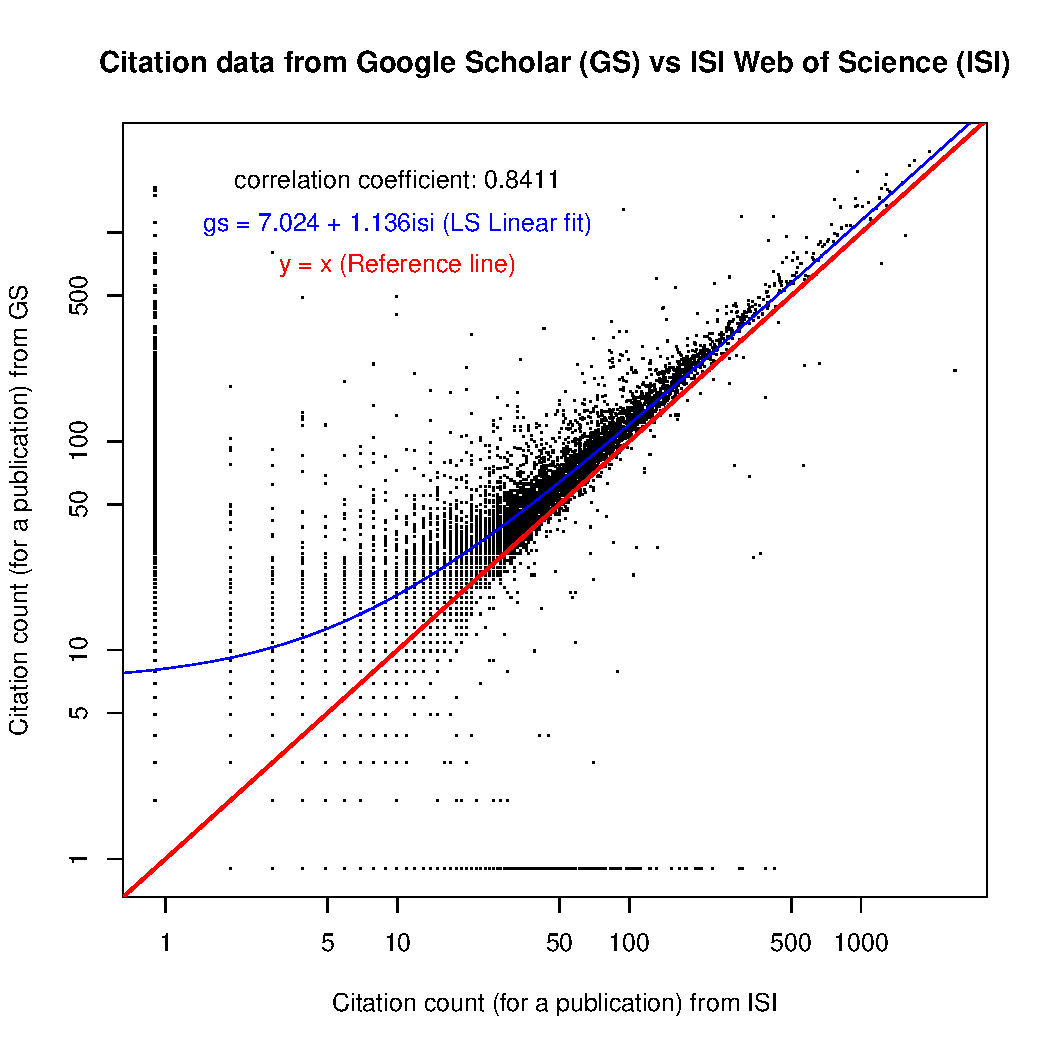
\includegraphics[width=1.0\columnwidth]{images/11_gs_vs_isi_cites.pdf}
  \caption{Citations (GS vs ISI)}\label{F:gs-vs-isi-cites}
\end{figure}

\begin{figure}[htb]
  \centering
    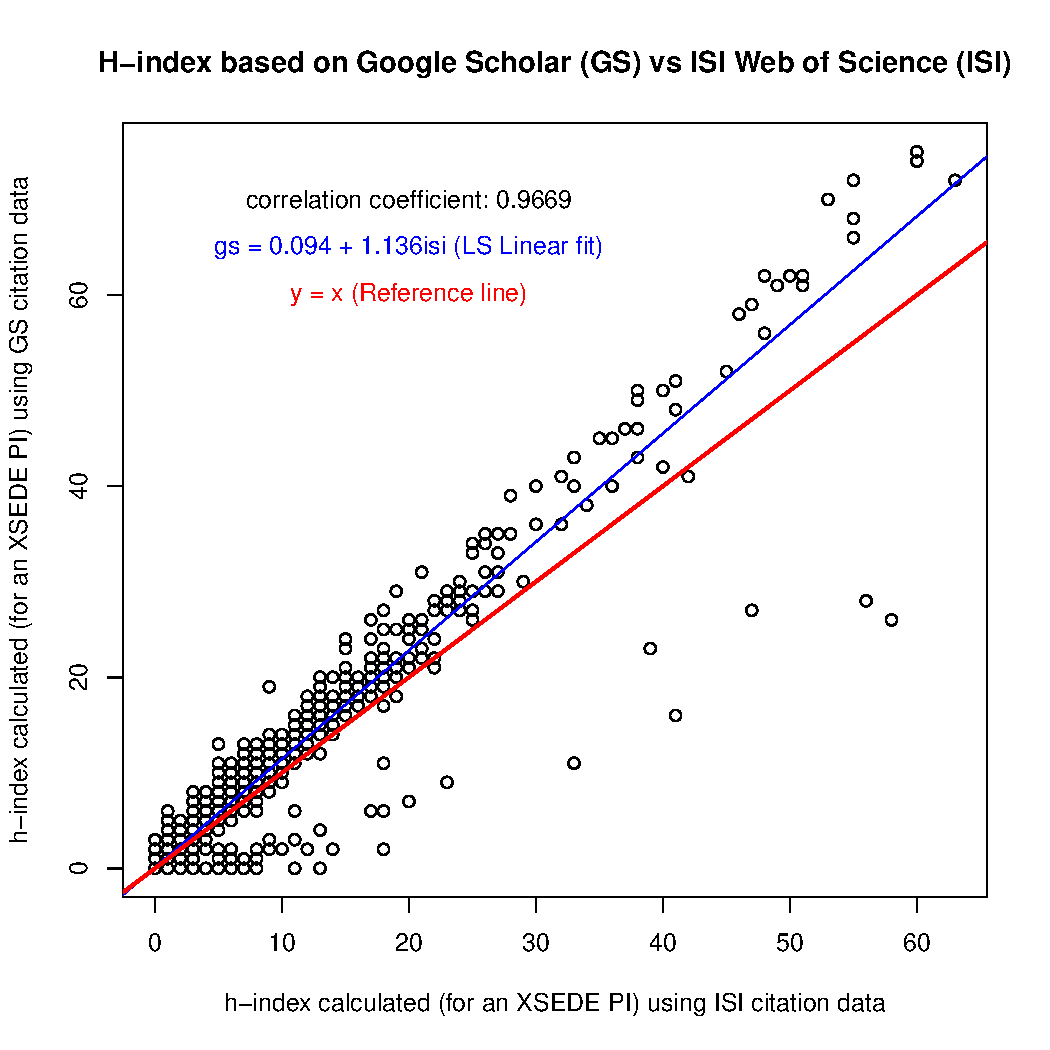
\includegraphics[width=1.0\columnwidth]{images/11_gs_vs_isi_hindex.pdf}
  \caption{H-index (GS vs ISI)}\label{F:gs-vs-isi-hindex}
\end{figure}

Figure \ref{F:gs-vs-isi-cites} shows the citation data from Google Scholar vs ISI Web of Science. Out of the 33861 data points, 20793 of them (61.4\%) have larger value in GS, 10315 (30.5\%) are the same, while 2753 (8.1\%) have larger value in ISI. 5287 (15.6\%) publications have zero citation found in ISI but non-zero in GS, 1253 (3.7\%) pubs have zero citaion in GS but non-zero in ISI. In general Google Scholar tends to have higher citation number.

Figure \ref{F:gs-vs-isi-hindex} shows that H-index obtained from Google Scholar data vs ISI data. Out of the 1462 data points, 663 of them (45.3\%) have larger value in GS, 677 (46.3\%) are the same, while 122 (8.3\%) have larger value in ISI.
52 (3.6\%) PIs have zero H-index computed from ISI data but non-zero from GS, 39 (2.7\%) for the reverse side. In general h-index calculated from Google Scholar data tends to be a bit higher.

In either case a high positive correlation is observed. The Pearson correlation coefficient are 0.84 and 0.97 respectively. The very strong correlation of the h-index values are mostly due to the fact that one of the two factors determining the h-index, the number of publications, stay the same for a perticular user.

Based on the study, while we don't have complete citation data from Google Scholar due to access restriction, we were able to use the ISI citation data to get very similar measures for most of the data especially for the h-index metric. Thus the following analyses are using the ISI citation data to further derive other metrics.


\section{Related Works}

Our choice of using publication as the basic unit to measure the impact is backed up by the fact that the bibliometric based criteria are the de-facto standards to measure the impact of research. For example, publication derived metrics are broadly used in Faculty recruit/promotion, institution ranking \cite{thomas1998institutional}.

For a publication, while usage based metrics are proposed by some research works \cite{Bollen:2007:MUM:1255175.1255273} \cite{Bollen:2008:TUI:1378889.1378928} \cite{bollen2009principal}, citation based metrics are probably still the standard and well accepted measure. In addition to the intuitive measures like number of publications and number of citations, h-index \cite{hirsch2005index} and g-index \cite{egghe2006theory} are other two popular metrics. Publication counts could be seen as a measure of the productivity, while citation counts measure the quality, or impact of the work published. As h-index and g-index calculate the metric by combining these data, they measure both the productivity and the quality, thus impact in general. For instance, nanoHub used these criteria to measure the impact of their project \cite{www-nanohubcite}. It defined a `citation' as a published work that cites/refers nanohub site or its related content, and `Secondary citation' as the citation received of the previously defined `citation'. Based on this, it analyzed the statistical distributions of the `citation' related data based on different criteria, e.g., author's organization; topic area - research, education; cited year; publication type; etc. The overall secondary citation and h-index are also computed to show the overall impact of the project.

There are existing tools to measure the metrics for individual users, e.g. Scholarometer \cite{kaur2012scholarometer} and Publish or Perish \cite{www-pop}. These could be potentially leveraged to analyze a relatively small group of users, e.g., the work \cite{bollen2011and} showing TeraGrid's impact based on limited data from one resource allocation meeting consisting of 112 PIs.
However, neither of the tools provides a scalable solution to the large community we are concerning which consists of over 20 thousands users.

While a more formal publication based metrics, either based on citation or usage, are still the most prevailing criteria, there are other proposals to include other measures. E.g., altmetrics \cite{www-altmetrics} proposes to include measures for dataset, code; as well as mentioning of a snippet of work via social networking; among others. We acknowledge these efforts as the trend of big data and social networking might suggest, however at the present there still lacks a standard and well established way to objectively derive measures based on these means.



\section{Evaluation}

\section{Discussion and Future Work}

This paper does not address the name ambiguity issue, which deserves dedicated research and in fact numerous research has been done tackling this issue. The root cause of this issue is that the metadata of the publications simply does not include enough information to distinguish similar user names. This is not a problem specific to our study but for the automated bibliometrics analysis in general, e.g., Google Scholar also include false positive publications in user profile but leave it to the user to curate the results to make it more accurate. In the future we will try to tackle the problem based on other available data - field of science, organization, funding data, co-author relationship etc. while conducting unsupervised machine learning techniques like k-means clustering.

As the ultimate approach is to let users vetting their publication list, we would try to include more such data. One pathway is to work with the XSEDE portal team while providing the publication data we have collected as a suggestion service, in the hope to provide more convenient way for users to quickly populate the vetted publications library. This is a work in progress now.

We have also started another similar activity, in which we wanted to extracting and parsing the publication data from past TeraGrid/XSEDE quarterly reports. These data, while not curated on per user basis, do have project level association information thus could serve quite well for most of our analysis.

Another activity we are also conducting is social networking related analysis among publications, users, projects, FOSes, etc. based on citation and co-authorship relations.



%%%%%%%%%%%%%%%%%%%%%%%%%%%%%%%%%%%%%%%%%%%%%%%%%%%%%%%%%%%%%%%%%%%%%%
% Acknowledgment
%%%%%%%%%%%%%%%%%%%%%%%%%%%%%%%%%%%%%%%%%%%%%%%%%%%%%%%%%%%%%%%%%%%%%%


\section*{Acknowledgement}

TAS Grant ... \todo{tas grant}

Some of the text published in this chapter is available form the
FutureGrid portal. The FutureGrid project is funded by the National
Science Foundation (NSF) and is led by Indiana University with
University of Chicago, University of Florida, San Diego Supercomputing
Center, Texas Advanced Computing Center, University of Virginia,
University of Tennessee, University of Southern California, Dresden,
Purdue University, and Grid 5000 as partner sites. This material is
based upon work supported in part by the National Science Foundation
under Grant No. 0910812. If you use FutureGrid and produce a paper or
presentation, we ask you to include the reference
\cite{las2010gce,las12fg-bookchapter}.

\bibliographystyle{IEEEtranS}
\bibliography{%
bib/references,%
bib/vonLaszewski-jabref,%
bib/image-refs,%
bib/cyberaide-cloud,%
bib/python}

%%%%%%%%%%%%%%%%%%%%%%%%%%%%%%%%%%%%%%%%%%%%%%%%%%%%%%%%%%%%
%\clearpage

%\appendix

\end{document}
